



\documentclass[journal]{IEEEtran}
\hyphenation{op-tical net-works semi-conduc-tor}
%%%%%%%%%%%%%%%%%%%%%%%%%%%%%%%%%%%%%%%%%%%%%%%%%%%%%%%%%%%%%%%%%%
%%%%%%%%%%%%%%%%%%%%%%%%%%%%%%%%%%%%%%%%%%%%%%%%%%%%%%%%%%%%%%%%%%
%%%%%%%%%%%%%%%%%%%%%%%%% PACKAGES %%%%%%%%%%%%%%%%%%%%%%%%%%%%%%%
%%%%%%%%%%%%%%%%%%%%%%%%%%%%%%%%%%%%%%%%%%%%%%%%%%%%%%%%%%%%%%%%%%
%%%%%%%%%%%%%%%%%%%%%%%%%%%%%%%%%%%%%%%%%%%%%%%%%%%%%%%%%%%%%%%%%%
\usepackage[T1]{fontenc}
\usepackage[utf8]{inputenc}
\usepackage{lmodern}
\usepackage[portuguese]{babel}
\usepackage{graphicx}
\usepackage{fancyhdr}
\usepackage{caption}
\usepackage{subcaption}
\usepackage{placeins}
\pagestyle{fancy}
\usepackage{color}
\usepackage{cancel}
\usepackage{steinmetz}
\graphicspath{{../images/}}

\newcommand{\HRule}{\rule{\linewidth}{0.5mm}}

\newcommand{\hRule}{\rule{\linewidth}{0.2mm}}

\begin{document}

\title{
\HRule \\
\Huge Introdução à Ciência dos Materiais \\
\huge Relatório Final
\HRule
}

\author{  \begin{tabular}{llr} \
    & & \\[0.05cm]
	\multicolumn{3}{ c }{Universidade de Brasília} \\
	\multicolumn{3}{ c }{\today} \\ \\
    Professora: & Palloma Vieira Muterlle & \\
    Alunos:& & \\
    & Juarez A.S.F                        & 11/0032829\\
    & Maria Cleuza Ornelas Parente        & 11/0036131\\
    & Rafaela Sano Machado 		& 11/0039360
      \end{tabular}
      }
\maketitle


\section{Discussão e Análise}

Consideramos para análise o gráfico \ref{fig:graph} 
a seguir.

\begin{figure}[!htp]
\centering
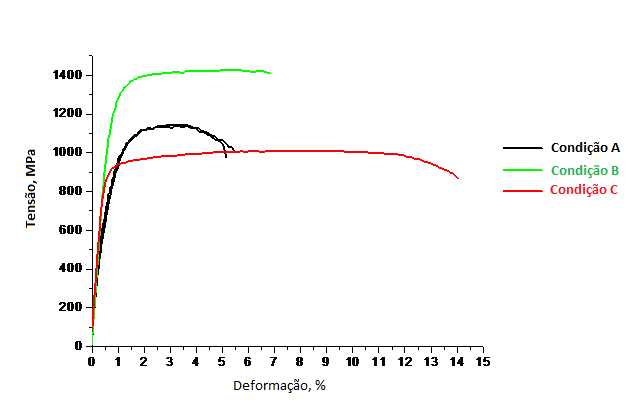
\includegraphics[scale=0.4]{../images/leGraph.png}
\caption{Diagrama tensão-deformação para 3 condições}
\label{fig:graph}
\end{figure}
\FloatBarrier

\subsection*{Questão 1}
Para o gráfico em análise vamos determinar alguns parâmetros:
\begin{itemize}
 \item \textbf{limite de escoamento : } 
 esse é o ponto até onde uma aproximação linear dada pela lei
 de Hooke é válida, em geral pode ser determinado pela tensão 
 que cause uma deformação de 0.02\%. Como não temos acesse a esse
 nível de precisão no gráfico dado, fazemos apenas uma estimativa 
 grosseira do real valor. Para as três condições dadas, temos:
 
 \begin{table}[!htp]
  \centering
  \begin{tabular}{|c|c|} \hline
  condição & limite de escoamento \\ \hline
  A & 1000 MPa \\ \hline
  B & 1300 MPa\\ \hline
  C & 800 MPa\\ \hline
  \end{tabular}
  \caption{limite de escoamento}
 \end{table}

  \item \textbf{Módulo de Elasticidade: } 
 é a constante K que relaciona a tensão($\sigma$) com a
 deformação ($\varepsilon$) na lei de Hooke $\sigma = k \varepsilon$
 durante a fase linear do escoamento. Para as três condições
 dadas, podemos estimar a constante pela fórmula $k = 
\frac{\Delta \sigma}{\Delta \varepsilon}$:
 \begin{table}[!htp]
  \centering
  \begin{tabular}{|c|c|} \hline
  condição & módulo de elasticidade($\approx$) \\ \hline
  A & $\frac{1000}{1\%} = 1000 \frac{KPa}{\%}$   \\ \hline
  B & $\frac{1300}{1\%} = 1300\frac{KPa}{\%}$\\ \hline
  C & $\frac{800}{1.5\%} = 533 \frac{KPa}{\%}$\\ \hline
  \end{tabular}
  \caption{módulo de elasticidade}
 \end{table}

   \item \textbf{Limite de Resistência à Tração: } 
corresponde à tensão máxima aplicada ao material antes da 
ruptura. Estimamos:
   
   \begin{table}[!htp]
  \centering
  \begin{tabular}{|c|c|} \hline
  condição & LRT \\ \hline
  A & 1100 KPa   \\ \hline
  B & 1400 KPa\\ \hline
  C & 950 KPa\\ \hline
  \end{tabular}
  \caption{limite de resistência à tração}
 \end{table}

    \item \textbf{Limite de Ruptura: } 

    \item \textbf{Ductilidade: }
    indica quanto o material deforma, em \%, antes da 
    fratura.
    
       \begin{table}[!htp]
  \centering
  \begin{tabular}{|c|c|} \hline
  condição & ductilidade \\ \hline
  A & 5\%   \\ \hline
  B & 7\% \\ \hline
  C & 14.5\% \\ \hline
  \end{tabular}
  \caption{ductilidade}
 \end{table}
    
\end{itemize}

\subsection*{Questão 2}
Classificamos agora as 3 condições em relação à:
\begin{itemize}
 \item \textbf{Rigidez:} relacionado ao módulo de elasticidade
 do material.
 C < A < B

 \item \textbf{Tenacidade:}Corresponde à capacidade do material de 
absorver energia até sua ruptura.

  A < B < C
 
 \item \textbf{Resiliência:} a capacidade de um material absorver 
energia quando este é deformado elasticamente

 C < A < B
 
 \item \textbf{Resistência e Fragilidade:}
  A condição mais frágil é A e a mais resistente à tração é C.
\end{itemize}

\subsection*{Questão 3}

A diferença entre a fratura do corpo de prova de um material frágil 
para um dúctil é o fato de nos materiais frágeis ocorrer fratura sem 
qualquer deformação apreciável, e esta deformação ocorre 
repentinamente e catastroficamente, sem qualquer aviso, ou seja, a 
propagação da trinca ocorre rápida e espontaneamente. Já os materiais 
dúcteis exibem tipicamente uma deformação plástica substancial com 
grande absorção de energia antes de ocorrer a fratura, porém, 
normalmente existe pouca ou nenhuma deformação plástica com baixa 
absorção de energia acompanhando uma fratura frágil. Além disso, outra 
característica da fratura dúctil é a extensa deformação plástica na 
vizinhança de uma trinca que está avançando, porém esta trinca tem 
propagação lenta e uma deformação plástica que permite ser prevenida.
\subsection*{Questão 4}

A dureza é a resistência do material à um esforço concentrado, 
pontual. Um mesmo material
apresenta resistência diferente à diferentes esforços e portanto a 
dureza não é uma medida absoluta. 
As diferentes durezas, a saber, Rockwell, Brinell e Vickers, aplicam 
diferentes esforços ao corpo de prova e são adequadas para situações
específicas.

\begin{itemize}
 \item \textbf{penetrador}:Na dureza Brinell o material é pressionado 
com uma esfera, na Vickers,
com uma pirâmide e na Rockwell, com um cone ou esfera. 
 \item \textbf{processo de medida:}
 \begin{itemize}
  \item  na dureza Rockwell a carga é 
aplicada em dois momentos e a diferença entre a profundidade de 
penetração em cada momento indica a dureza. 
\item na dureza Brinell mede-se a razão entre a carga aplicada e a 
área impressa no corpo de prova.
\item na Vickers o processo é baseado na resistência do material à 
penetração de uma pirâmide
 \end{itemize}

\end{itemize}

\subsection*{Questão 5}


As etapas do processo de preparação metalográfica são: escolher o 
local da amostra a observar; corte no material para a obtenção de uma 
superfície tão plana quanto possível; polimento, para remover as 
irregularidades da superfície a fim de obter uma superfície plana à 
escala que será utilizada na observação; ataque químico 
(contrastação), cuja escolha para este procedimento é condicionada 
pelo material a observar e pelas condições de observação.
A importância das etapas do processo de preparação metalográfica 
consiste em analisar ou explicar o comportamento e as propriedades de 
uma peça metálica, pelo fato de permitir conhecer a estrutura do 
material e, também, os seus constituintes micro-estruturais, assim 
como sua a morfologia e a sua distribuição.
\subsection*{Questão 6}


A liga de aço 1020 era maior parte branca com pequenos grãos escuros, 
e isto ocorre pelo fato da liga ter baixa taxa de carbono na sua 
composição. A parte clara é composta pela ferrita, e os grãos escuros 
são compostos pela perlita, e há traços de cementita também. Já a liga 
1045 é escura pelo fato de ter alta porcentagem de carbono em sua 
composição, e esta parte escura é a perlita e as estruturas brancas 
são compostas pela ferrita. Os grãos são finos, longos e pequenos.
\subsection*{Questão 7}

A liga de aço 1020, que têm baixa dureza pelo fato de ter baixa liga, 
reagiu de forma positiva após o experimento, pois houve aumento da 
dureza em decorrência da formação da estrutura martensítica.
Na aula 
prática, esta liga reagiu de forma positiva após o experimento, pois 
houve aumento da dureza em decorrência da formação da estrutura 
martensítica. O aço 1020 tem 0,2\% de carbono em sua composição e 
possui excelente plasticidade e soldabilidade.
A liga de aço 1045 também tem baixa dureza e baixa concentração 
relativa de carbono: 0,45\%. No experimento, houve aumento da dureza 
deste material em decorrência do refinamento dos grãos e dos alívios 
de tensões da liga. Como houve resfriamento da austenita, esta se 
transformou em um novo constituinte do aço, a martensita, cuja 
concentração é proporcional à dureza, e isso fez com que houvesse 
aumento da dureza do aço.


%@@@@@@@@@@@@@@@@@@@@@@@@@@@@@@@@@@@@@@@@@@@@@@
%@@@@@@@@@@@@@@       REFERÊNCIAS     @@@@@@@@@@@@@@@@@@@@@@
%@@@@@@@@@@@@@@@@@@@@@@@@@@@@@@@@@@@@@@@@@@@@@@
\begin{thebibliography}{9}    
    
    \bibitem{rafaela}
    GUY A. G. 
    \emph{Ciência dos Materiais}. 
    São Paulo, 1ª Edição LTC, 
    1980.

\bibitem{rafaela2}
FERRAZ H. O 
\emph{Aço Na Construção Civil, Revista Eletrônica de Ciências}.
22ª Edição, 2003.

    \bibitem{rafala3}
  GARCIA, A.: SPIM, J.A.: SANTOS, C.A.
  \emph{Ensaios dos Materiais}. 
    LTC, Rio de Janeiro,  1ª Edição, 2000.
   
\end{thebibliography}
\end{document}


